\section{Introduction}
%%%%%%%%%%%%%%%%%%%%%%

% Paragraph 1: why cryptographic functions are important
Cryptography has found itself at the core of secure modern technology and both plays a key role in securing communications and
is imperative to many modern systems and applications.
From data integrity to authentication and online banking to messaging friends, cryptography is everywhere.
Well-known cryptographic libraries, such as OpenSSL~\cite{openssl}, are widely used not only to generate
TLS certificates and validate certificate information, but also to implement cryptography in general purpose applications.
Despite their universal benign usage, cryptographic functions are also heavily used in malware and
to evade security protocols. In recent ransomware attacks ~\cite{wannacry,petya},
cryptographic functions have been used to encrypt a victim's information and later
asked to pay ransom in exchange of recovering their files and information.

% Paragraph 2: Motivation behind indentification 
On the one hand, the usage of cryptographic functions makes it easier to carry out
secure and private operations, and on the other hand, its malicious usage by bad actors makes
it harder for cryptography and security experts to perform forensic analyses and reverse engineer code.
Hence, the ability to automatically identify or detect the presence of cryptographic functions
in binary applications can be a crucial part of the security experts' arsenal.
It can assist in binary analysis to give a better depiction of how the
functions work.  Determining the type of cryptographic function in a
binary can help to pinpoint the existence of a malicious
payload~\cite{yan2008revealing} and also help cryptographic experts identify potentially insecure protocols or implementations (or those that require more manual analysis).
%Finally, oftentimes malware and ransomware use
%similar cryptographic functions with some minor changes. For example, there are
%different versions of the TeslaCrypt ransomware~\cite{teslacrypt}.
%Identifying one piece of ransomware via an automatic detection mechanism can help to
%identify other versions and thus save time and resources that could be better devoted to implementing
%effective prevention mechanisms.

\begin{figure}[t]
  \centering
  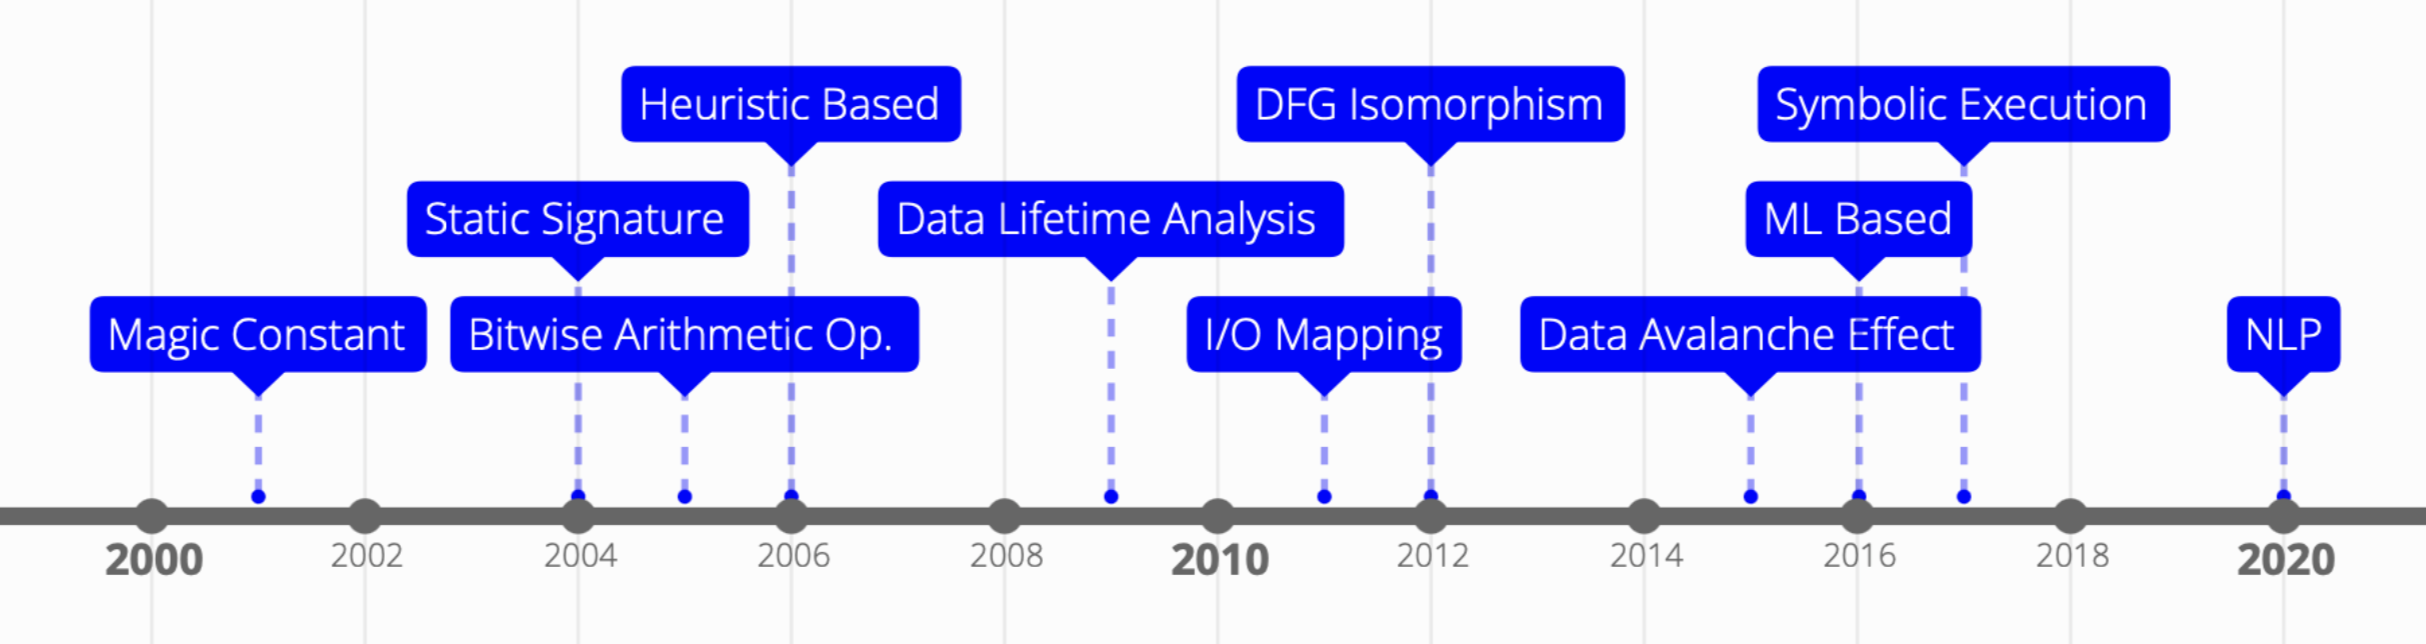
\includegraphics[width=0.95\textwidth,keepaspectratio]{ch-cryptobinary/figure/Crypto_timeline.png}
  \caption{Evolution of cryptographic function identification techniques}
  \label{fig:cryptobinary-timeline}
\end{figure}

%%4 Paragraph 3: Challenges
%However, cryptographic function identification has its own sets of challenges.
%Binaries can be obfuscated in a variety of ways, such as control-flow flattening,
%data-splitting, data-aggregation, and inclusion of bogus control-flow. In addition,
%simple cryptographic algorithms can be implemented in a variety of ways, hence
%detection mechanism that may work on one variation may fail on its more complicated (or more simplified) implementations. Malware authors also generate packed binaries to evade
%any possible detection.


While general purpose binary analysis and function identification techniques are themselves broad and thriving areas that could potentially solve these problems, a variety of work across industry and academia has focused on solving these challenges more specifically: developing techniques and tools that are uniquely tailored to identifying \textit{cryptographic primitives} in binary applications.  This allows researchers to often provide better results in different domains, leveraging cryptography-specific features.
% Paragraph 4: landscape
Cryptographic functions tend to have many mathematical computations,
nested loops, and exclusive input-output mappings which are distinct from
non-cryptographic functions and can thus be useful as a means of identification. 
% \autoref{fig:cryptobinary-timeline} shows a timeline of various techniques and approaches used in cryptographic function identification research to date.
%\priyam{taken it to the background}
Harvey et al.~\cite{harvey2001cipher} first utilized magic constants to identify
cryptographic primitives in 2001. Later works focused on signature
based detection mechanisms. However, due to the limitations of signature
based approaches, subsequent work placed a greater emphasis on heuristic based detection, such as
identification of basic blocks, instruction patterns, etc. With the
popularization of modern machine learning algorithms, newer works utilized
deep learning and AI to extract cryptographic features from a binary.
%We discuss these various approaches in depth in Section~\ref{sec:features}.

Unfortunately, while there has been a wealth of work in the space, it has generally failed to keep up with modern cryptographic
innovations and applications, as well as current software engineering and optimization techniques.
This can be difficult to notice as there is no standardized benchmarking or comparison framework, and individual works tend to test on algorithms that they are best at identifying, while neglecting those they cannot.
Additionally, as many techniques are tailored for specific cryptographic algorithms, architectures, or settings, which change rapidly over time, reproducing past results can be challenging, making it difficult to provide comparisons across the growing landscape as well.
%Additionally, while there have been some surveys on encryption algorithms~\cite{mushtaq2017survey} and ransomware detection/mitigation~\cite{begovic2023cryptographic, mcintosh2021ransomware, smith2022machine}, these works do not investigate the capabilities of different detection tools or the gaps in the selection of algorithms.

Given how important these tools and techniques can be for both researchers and practitioners, we aim to reproduce and replicate all existing tools to date in this domain.  In this endeavor, we also offer a comprehensive analysis that categorizes and discusses the existing body of work, highlighting the strengths, weaknesses, and techniques employed.
We also seek to help drive future research in the area by identifying potential challenges and various factors that may influence performance.
%highlighting a taxonomy of modern cryptographic algorithms and discussing features that we think could be leveraged for identification. 
To help provide for a more even comparison of existing and future work, and to identify gaps that are in need of future research, we create a benchmarking framework featuring a number of modern cryptographic primitives and applications. We then use this framework to evaluate existing work.
Finally, throughout the paper, we discuss and motivate a variety of open research problems in the space.

\subsection{Our Contributions}
Our primary contributions are:

\begin{itemize}[noitemsep,topsep=0pt]

%\item We present a systematic study of cryptographic function identification
%approaches, discussing various techniques that have been leveraged, as well as their strengths and weaknesses.

\item We conduct a thorough examination of cryptographic function identification methods, exploring the range of techniques utilized and evaluating their respective strengths and limitations.

%\item We highlight a taxonomy of modern cryptographic algorithms and discuss various features of cryptographic algorithms that can be leveraged for identification purposes.
%\item We highlight a number of features of cryptographic algorithms that can be leveraged for identification purposes.

%\item We discuss a number of challenges that modern tool developers and researchers face in the space from a software and implementation perspective, such as optimizations and non-standard implementations.

\item We create a standardized suite of performance metrics and benchmarks to evaluate the effectiveness
of current detection mechanisms and analyze existing tools based on this suite.

\item We conduct comprehensive replication and reproduction studies on all existing work.

\item We provide an in-depth analysis of our findings and categorize the tools according to their performance across various dimensions.

\item Based off of this analysis and our study of existing work, we discuss the research gaps in this domain and propose directions for future work.

%\item We propose a simple tool to identfy cryptographic functions based on the program state change \priyam{TODO: update based on the eval status}
  
%\item We present a comprehensive framework to understand the scalability and
%impact of dynamic analysis in detection mechanisms. \clg{Is this one left over from your thesis?  I'm not sure how it fits in overall with the paper.}
%\priyam{we can get rid of this part}

\end{itemize}

% \subsection{Chapter Organization} The outline of our paper is as follows.
% In Section~\ref{sec:taxonomy} we present our taxonomy of cryptographic algorithms, and in Section~\ref{sec:features} we discuss the various features of cryptographic algorithms that have been used for identification.
% In Section~\ref{sec:detection} we analyze different detection techniques and their strengths and weaknesses, and in Section~\ref{sec:challenges} we enumerate the inherent challenges in detecting and classifying cryptographic code in real-world applications.
% In Sections~\ref{sec:framework} and~\ref{sec:evaluation} we introduce our benchmarking framework and run existing tools on it to generate a fair comparison among existing work and highlight gaps in coverage.

